A common operational approach that water utilities use to address water quality concerns is flushing, which 
is the purging of water from the distribution network via a fire hydrant or blow-off port. 
Many utilities flush water mains following maintenance work 
or in response to customer complaints. Flushing can remove the sources 
of poor water quality (e.g., pipe corrosion, bio-film microorganisms), as well 
as loose or suspended material that has accumulated in low-flow portions or 
dead-ends of the distribution system. It is a response option that can be undertaken 
relatively quickly after a contamination incident, and it can be made more efficient through 
the careful selection of where to implement flushing activities. This chapter describes 
the \code{flushing} subcommand in WST that assists in the identification of effective 
hydrant locations to flush in order to remove contaminated water and the valves to close 
in order to direct the contaminated water towards the hydrants. 

A flowchart representation of the \code{flushing} subcommand is shown in Figure \ref{fig:flushing-flowchart}. 
The \code{flushing} subcommand employs an iterative process that combines contaminant transport, impact assessment 
and optimization. The optimization process identifies a set of flushing activities 
that are simulated in the contaminant transport process and evaluated 
based upon the impact assessment process. Since the \code{flushing} subcommand relies 
on the \code{tevasim} and \code{sim2Impact} subcommands, their required input 
is also required for the \code{flushing} subcommand. In addition, the sensor network 
design used to detect the contamination incident(s) and the flushing characteristics 
are required inputs. The utility network model is defined by a EPANET 2.00.12 INP file, 
while the rest of the input can be specified in the \code{flushing} WST configuration file.

\begin{figure}[h]
  \centering
  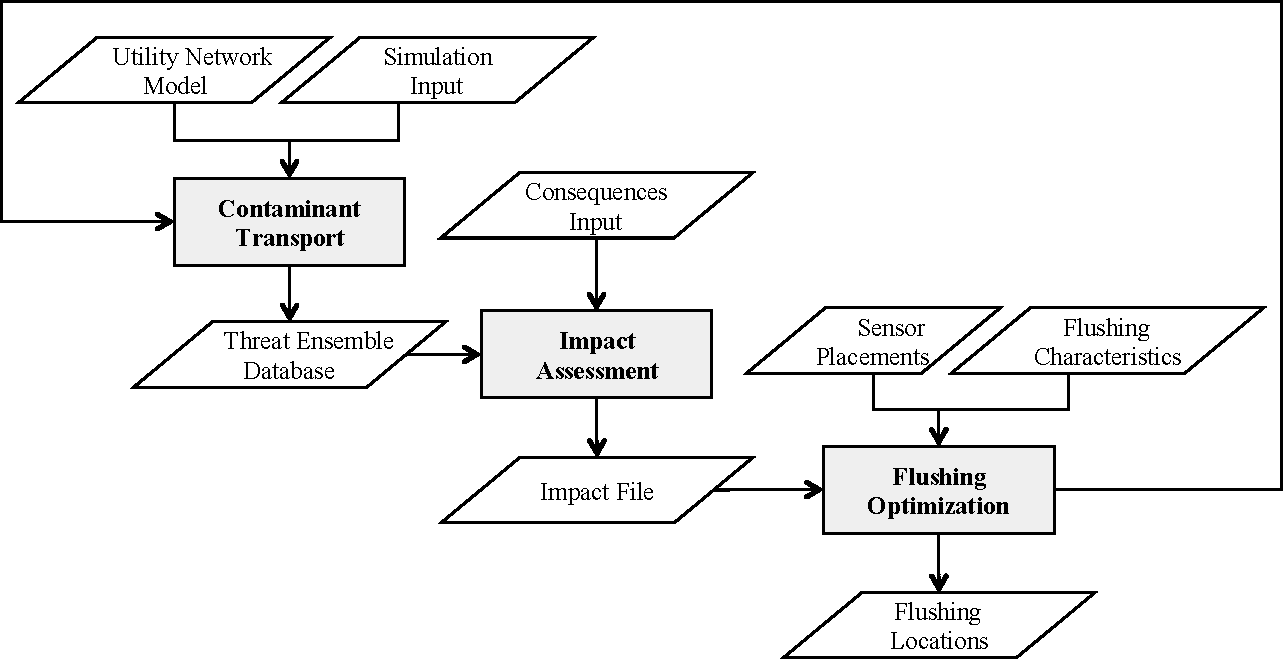
\includegraphics[scale=0.75]{graphics/flushing_flowchart.pdf}
  \caption{Flushing response simulation flowchart.}
  \label{fig:flushing-flowchart}
\end{figure}

\section{Flushing Formulation}\label{flushing_formulations}
The flushing problem formulation can be summarized 
as selecting a set of hydrant locations to flush and valves to close 
that minimizes the average impact of all contamination incidents 
given a set of potential hydrant locations to flush and valves to close. 
The mathematical formulation can be written as follows:
\begin{align}
\textrm{  minimize } \qquad &\dfrac{1}{A} \sum_{a \in {A}} d_{a,\max} \label{eqn:flushing} \\
\textrm{subject to } \qquad &\sum_{h\in H}y_{h} \leq H_{\max} \label{eq:flushing_2} \\
&\sum_{v\in V}y_{v} \leq V_{\max} \label{eq:flushing_3} \\  
&y_{h} \in \{0,1\} &&\forall h\in H \label{eq:flushing_4} \\
&y_{v} \in \{0,1\} &&\forall v\in V \label{eq:flushing_5}
\end{align}
where $A$ represents a set of contamination incidents, 
$d_{a,\max}$ defines the maximum impact of the contamination incident $a$, 
$H$ represents the set of potential hydrant locations,
$y_h$ is a binary variable which is 1 if node $h$ is selected as a flushing location, 
$H_{\max}$ is the maximum number of hydrant locations,
$V$ represents the set of potential valve locations,
$y_v$ is a binary variable which is 1 if node $v$ is selected as a valving location and 
$V_{\max}$ is the maximum number of valve locations. The maximum impact of a contamination
incident, $d_{a,\max}$, is the total impact across the entire network at the end of the simulation 
assuming that the contaminant was not detected by a sensor, and no interventions to reduce 
impacts were implemented. This value is found in the -1 entry of the impact file. 

For this problem, hydrants are assumed to be located at any user-defined nodes in the network. 
In addition, valves are assumed to be located on any user-defined pipes in the network.  

\section{Flushing Solvers}\label{flushing_solvers}
The flushing problem is solved through an iterative optimization process which 
selects different sets of hydrant and valve locations and evaluates their effectiveness
in minimizing the impact of a set of contamination incidents. Two optimization 
methods, an evolutionary algorithm and a network solver, are available in WST to solve this problem. 
Each solver is explained in more detail in the following subsections. 

\subsection{Evolutionary Algorithm}\label{coliny_ea}
The evolutionary algorithm (EA) included with DAKOTA, Coliny EA, is used in the 
optimization routine for the \code{flushing} subcommand. 
Additional information on DAKOTA/Coliny solvers can be found at 
\url{http://dakota.sandia.gov/docs/dakota/5.2/html-ref/index.html}
and in the DAKOTA user manual \citep{DakotaUserManual}.  
The random number generator used in Coliny EA is platform dependent.  
This can result in slight variations in the solution.

To design an EA, the parameter space for the optimization problem 
is first encoded into a string of numbers. This encoded 
representation of the problem is called a genetic string, where each 
element of the genetic string represents one parameter. 
When the EA is used with the \code{flushing} subcommand, the parameter space is defined by the number 
of flushing and valve closure locations. Each location is assigned a sequential 
integer that represents a feasible location within the EPANET network. The final EA solution 
is reported based on the EPANET node/pipe IDs.

The EA has several solver options that define how the EA evolves. These options can be set in the 
\code{[solver][options]} sections of the \code{flushing} WST configuration file and are specific to the Coliny EA solver. 
The EA evolves an initial genetic strings of size \code{[population\_size]} 
that is set based on \code{[initialization\_type]} using the following steps:
\begin{enumerate}
\item Evaluation: Evaluate the solution for each genetic string. This involves function 
calls to the \code{tevasim} and \code{sim2Impact} subcommands for each string to define the impact value.  
\item Breeding: Select two members of the population based on fitness. The 
probability of selection is based on \code{[fitness\_type]}.  
\item Crossover: Crossover two members based on \code{[crossover\_type]} and \code{[crossover\_rate]}.
\item Mutation: Mutate the two members based on \code{[mutation\_type]} and \code{[mutation\_rate]}.
\item Steps 2-4 are repeated until the entire population has been changed.
\item Replacement: After a new population is created, the old population is 
replaced by the current population while keeping the highest ranked string 
(elitist = 1 replacement option).
\end{enumerate}
Steps 1-6 are repeated until \code{[max\_iterations]} or \code{[max\_function\_evaluations]} criteria is met. 

\subsection{Network Solver}\label{coliny_statemachine}

The network solver used in WST is a network-constrained, derivative-free local search optimization algorithm. 
It is a discrete analog-to-pattern search. The allowable moves are to adjacent nodes (or pipes), rather than moves in the 
continuous space. This approach provides local refinement of candidate solutions. The valid moves include
removing a node (or pipe) location and replacing it with one anywhere in the network. Two forms of the network solver can be 
used: with and without initial starting points. The initial starting points are node (or pipe) locations in the network
in which the algorithm should begin its local search. If these points are not supplied to the algorithm, 
then it reduces to a greedy placement algorithm. Convergence is met when no remaining moves improve the solution.

\subsection{Flushing Optimization for Large Problems}

The iterative optimization process used for flushing requires numerous 
simulations of the network hydraulics and water quality. Computational run time depends on several factors, including 
the size of the network model, 
the number of possible contamination incidents, 
the number of feasible flushing locations 
and the solver options. For the network solver,the computational run time also depends on the network model
geometry surrounding the local search region. For large flushing optimization problems, several techniques can be used to 
decrease the computational run time. These options include running multiple instances of the underlying 
simulation in parallel, setting a stop time criteria and skeletonizing the network model.  

\subsubsection{Parallelization}

The Dakota coliny\_ea and StateMachineLS solvers both include an option to set 
the number of threads used to perform the simulations.   
This option is specified in \code{[solver][threads]}, as shown below. It should be 
set to the number of threads that are available for the simulation. The default value is 1.  
If an integer greater than 1 is specified, Dakota will run that many threads.
The expected efficiency of parallelization is nearly linear with the number of 
threads (up to the number of processor cores in the computer).

\begin{unknownListing}
solver:
  type: coliny_ea 
  threads: 2
\end{unknownListing}

\subsubsection{Stop time criteria}

If a solution needs to be identified within a certain amount of time, a simulation stop time 
criteria can be defined. This option causes the solver to terminate after a 
specified time, even if the underlying algorithm has not converged to an optimal solution.  
The stop time criteria is included with both the Dakota coliny\_ea and 
StateMachineLS solvers, and it is specified in \code{[solver][options][misc\_options]}, as 
shown below. The max\_time has to be given in seconds. As the optimization 
algorithms only check the elapsed time once per major iteration, the actual 
solver run time will be slightly longer than the specified maximum run time.  
When the optimization process is cut off prematurely, the best solution 
obtained so far is reported to the user.

\begin{unknownListing}
solver:
  type: StateMachineLS  
  options: 
    misc_options: "'max_time=10'"
\end{unknownListing}

\subsubsection{Skeletonization}

To reduce the size of the network model, possible contamination incidents and the number of 
feasible flushing locations, the user can skeletonize the problem and evaluate 
the results on the full network model. WST includes a utility script, spotSkeleton,  
that can be used to skeletonize network models (See Executable Files Section ~\ref{skelExecutable}).  
Network models are skeletonized based on a pipe diameter threshold. The executable, spotSkeleton,  
creates a new EPANET input (inp) file and a related map file.  
The map file associates the nodes in the skeletonized network model (upscaled nodes)  
to the nodes in the original network model (downscaled nodes). When  
working with a skeletonized network model, other aspects of the flushing problem also  
need to upscaled based on the skeletonization map. These include: the injection location(s)  
and strength of the contamination incident(s), the population at each node, the sensor  
placement, the feasible flushing locations and the initial points for the optimization  
solver. For example, if Nodes 1, 2, 3 and 4 in the original network model are  
represented by Node 2 in the skeletonized network model, then a sensor placed at  
Node 4 in the original network model should be placed at Node 2 in the skeletonized  
network model. 

After flushing optimization is run on the skeletonized network model, the  
solution can then be evaluated or refined using the original network model.  
To evaluate the current solution, the locations on the skeletonized network 
should be listed as the only feasible flushing locations  
in the original network model and the EVALUATE solver option should be used (See Example ~\ref{flushing_ex3}).   
To refine the current solution, downscale the locations on the skeletonized network
and use those original network nodes as the only feasible flushing locations  
in a second optimization. In this refinment, the solver type and  
solver options can be different for the first and second optimization.

\section{\code{flushing} Subcommand}

The \code{flushing} subcommand is executed using the following command line:
\begin{unknownListing}
wst flushing <configfile> 
\end{unknownListing}
where \code{configfile} is a WST configuration file in the YAML format. 

The \code{---help} option prints information about this subcommand, such as usage,
arguments and a brief description:
\begin{unknownListing}
wst flushing --help
\end{unknownListing}

\subsection{Configuration File}

The \code{flushing} subcommand generates a template configuration file using the following command line:

\begin{unknownListing}
wst flushing --template <configfile>
\end{unknownListing}

The \code{flushing} template configuration file is shown in Figure \ref{fig:flushing_template}.  
Brief descriptions of the options are included in the template after the \# sign.  

\begin{figure}[p!]
  \unknownInputListing{examples/flushing_config.yml}{}{1}{50}
  \caption{The \code{flushing} configuration template file.}
  \label{fig:flushing_template}
\end{figure}

\subsection{Configuration Options}

Full descriptions of the WST configuration options used by the \code{flushing} subcommand are listed below.
\begin{description}[topsep=0pt,parsep=0.5em,itemsep=-0.4em]
  \item[{network}]\hfill
  \begin{description}[topsep=0pt,parsep=0.5em,itemsep=-0.4em]
    \item[{epanet file}]\hfill
\\ The name of the EPANET 2.00.12 input (INP) file that defines the water distribution
                network model.
                
                Required input.
  \end{description}
  \item[{scenario}]\hfill
  \begin{description}[topsep=0pt,parsep=0.5em,itemsep=-0.4em]
    \item[{location}]\hfill
\\A list that describes the injection locations for the contamination scenarios.
                The options are: (1) ALL, which denotes all nodes (excluding tanks and reservoirs)
                as contamination injection locations; (2) NZD, which denotes all nodes with
                non-zero demands as contamination injection locations; or (3) an EPANET node ID, 
                which identifies a node as the contamination injection location. This allows 
                for an easy specification of single or multiple contamination scenarios.
                
                Required input unless a TSG or TSI file is specified.
    \item[{type}]\hfill
\\The injection type for the contamination scenarios. The options are MASS, CONCEN, FLOWPACED or SETPOINT. 
                See the EPANET 2.00.12 user manual for additional information about source types \citep{EPANETusermanual}.
                
                Required input unless a TSG or TSI file is specified.
    \item[{strength}]\hfill
\\The amount of contaminant injected into the network for the contamination scenarios.  
                If the type option is MASS, then the units for the strength are in mg/min. 
                If the type option is CONCEN, FLOWPACED or SETPOINT, then units are in mg/L.
                
                Required input unless a TSG or TSI file is specified.
    \item[{species}]\hfill
\\The name of the contaminant species injected into the network. This is the name of a single species. 
                It is required when using EPANET-MSX, since multiple species might be simulated, but
                only one is injected into the network. For cases where multiple contaminants are injected,
                a TSI file must be used.
                
                Required input for EPANET-MSX unless a TSG or TSI file is specified.
    \item[{start time}]\hfill
\\The injection start time that defines when the contaminant injection begins. 
                The time is given in minutes and is measured from the start of the simulation. 
                For example, a value of 60 represents an injection that starts at hour 1 of the simulation.
                
                Required input unless a TSG or TSI file is specified.
    \item[{end time}]\hfill
\\The injection end time that defines when the contaminant injection stops.				
                The time is given in minutes and is measured from the start of the simulation.
                For example, a value of 120 represents an injection that ends at hour 2 of the simulation.
                
                Required input unless a TSG or TSI file is specified.
    \item[{tsg file}]\hfill
\\The name of the TSG scenario file that defines the ensemble of contamination
                scenarios to be simulated. Specifying a TSG file will
                override the location, type, strength, species, start and end times options specified in
                the WST configuration file. The TSG file format is documented in File Formats Section \ref{formats_tsgFile}.
                
                Optional input.
    \item[{tsi file}]\hfill
\\The name of the TSI scenario file that defines the ensemble of contamination
                scenarios to be simulated. Specifying a TSI file will
                override the TSG file, as well as the location, type, strength, species, start and end time options specified in
                the WST configuration file. The TSI file format is documented in File Formats Section \ref{formats_tsiFile}.
                
                Optional input.
    \item[{signals}]\hfill
\\Name of file or directory with information to generate 
                or load signals. If a file is provided the list of inp tsg tuples
                 will be simulated and the information stored in signals files. If
                a directory with the signals files is specified, the signal files will
                be read and loaded in memory. This input is only valid for the uq
                subcommand and the grabsample subcommand with probability based formulations.

                Optional input.
    \item[{msx file}]\hfill
\\The name of the EPANET-MSX multi-species file that defines the multi-species reactions to
                be simulated using EPANET-MSX.
                
                Required input for EPANET-MSX.
    \item[{msx species}]\hfill
\\The name of the MSX species whose concentration profile will be saved by the EPANET-MSX simulation
                and used for later calculations.
                
                Required input for EPANET-MSX.
    \item[{merlion}]\hfill
\\A flag to indicate if the Merlion water quality
                simulator should be used. The options are true or false. 
                If an MSX file is provided, EPANET-MSX will be used.
                
                Required input, default = false.
  \end{description}
  \item[{impact}]\hfill
  \begin{description}[topsep=0pt,parsep=0.5em,itemsep=-0.4em]
    \item[{erd file}]\hfill
\\The name of the ERD database file that contains the 
                contaminant transport simulation results. It is 
                created by running the \code{tevasim} subcommand.
                Multiple ERD files (entered as a list, i.e., [<file1>, <file2>]) can be combined to
                generate a single impact file. This can be used to combine
                simulation results from different types of contaminants, in
                which the ERD files were generated from different
                TSG files.
                
                Required input.
    \item[{metric}]\hfill
\\The impact metric used to compute the impact file. Options
                include EC, MC, NFD, PD, PE, PK, TD or VC. One impact file 
                is created for each metric selected. These metrics are 
                defined in Section \ref{impact_measures}.
                
                Required input.
    \item[{tai file}]\hfill
\\The name of the TAI file that contains health impact information. 
                The TAI file format is documented in File Formats Section \ref{formats_taiFile}.
                
                Required input if a public health metric is used (PD, PE or PK).
    \item[{response time}]\hfill
\\The number of minutes that are needed to respond to the
                detection of a contaminant. This represents the time that it takes
                a water utility to stop the spread of the contaminant in the network and 
                eliminate the consumption of contaminated water. As the response time increases,
                the impact increases because the contaminant affects the network
                for a greater length of time.  
                
                Required input, default = 0 minutes.
    \item[{detection limit}]\hfill
\\The minimum concentration that must be exceeded before a sensor can detect a contaminant.
                There must be one threshold for each ERD file. The units of
                these detection limits depend on the units of the contaminant
                simulated for each ERD file (e.g., number of cells of a
                biological agent).  
                
                Required input, default = 0.
    \item[{detection confidence}]\hfill
\\The number of sensors that must detect an incident before
                the impacts are calculated.  
                
                Required input, default = 1 sensor.
  \end{description}
  \item[{flushing}]\hfill
  \begin{description}[topsep=0pt,parsep=0.5em,itemsep=-0.4em]
    \item[{detection}]\hfill
\\The sensor network design used to detect contamination scenarios. The
                sensor locations are used to compute a detection time for each 
                contamination scenario. The options are a list of 
                EPANET node IDs or a file name which contains a list of EPANET node IDs.
                
                Required input.
    \item[{flush nodes}]\hfill
    \begin{description}[topsep=0pt,parsep=0.5em,itemsep=-0.4em]
      \item[{feasible nodes}]\hfill
\\A list that defines the nodes in the network that can be flushed. 
                The options are: (1) ALL, which specifies all nodes as feasible flushing locations;
                (2) NZD, which specifies all non-zero demand nodes as feasible flushing locations;
                (3) NONE, which specifies no nodes as feasible flushing locations;
                (4) a list of EPANET node IDs, which identifies specific nodes as feasible flushing locations; or
                (5) a filename, which references a space or comma separated file containing a list of 
                specific nodes as feasible flushing locations.
                
                Required input, default = ALL.
      \item[{infeasible nodes}]\hfill
\\A list that defines the nodes in the network that cannot be flushed. 
                The options are: (1) ALL, which specifies all nodes as infeasible flushing locations;
                (2) NZD, which specifies all non-zero demand nodes as infeasible flushing locations;
                (3) NONE, which specifies no nodes as infeasible flushing locations;
                (4) a list of EPANET node IDs, which identifies specific nodes as infeasible flushing locations; or
                (5) a filename, which references a space or comma separated file containing a list of 
                specific nodes as infeasible flushing locations. 
                
                Optional input, default = NONE.
      \item[{max nodes}]\hfill
\\The maximum number of node locations that can be flushed simultaneously in the
                network. The value is a nonnegative integer or a list of
                nonnegative integers. When a list is specified, the optimization
                will be performed for each number in this list. For example, a value of 
                3 means that a maximum of 3 node will be identified as flushing locations 
                during the optimization process.
                
                Required input.
      \item[{rate}]\hfill
\\The flushing rate for each node location to be flushed. A new demand pattern 
                will be created using this rate for the node. The value is a nonnegative integer. 
                For example, a value of 800 means that an additional demand of 800 gpm is applied 
                at a particular node. This rate is applied to all flushing locations identified 
                in the optimization process.
                
                Required input.
      \item[{response time}]\hfill
\\The time in minutes between the detection of a contamination incident and 
                the start of flushing. The value is a nonnegative integer. For example, 
                a value of 120 represents a 120 minutes or a 2 hour delay between 
                the time of detection and the start of flushing.
                
                Required input.
      \item[{duration}]\hfill
\\The length of time in minutes that flushing will be simulated at a particular node. 
                The value is a nonnegative integer. For example, a value of 240 means that  
                flushing would be simulated at a particular node for 4 hours. This duration 
                is applied to all flushing locations identified in the optimization process.
                
                Required input.
    \end{description}
    \item[{close valves}]\hfill
    \begin{description}[topsep=0pt,parsep=0.5em,itemsep=-0.4em]
      \item[{feasible pipes}]\hfill
\\A list that defines the pipes in the network that can be closed. 
                The options are: (1) ALL, which specifies all pipes as feasible pipes to close;
                (2) DIAM min max, which specifies all pipes with a specific diameter as feasible pipes to close;
                (3) NONE, which specifies no pipes as feasible pipes to close;
                (4) a list of EPANET pipe IDs, which identifies specific pipes as feasible pipes to close; or
                (5) a filename, which references a space or comma separated file containing a list of 
                specific pipes as feasible pipes to close. 
                
                Required input, default = ALL.
      \item[{infeasible pipes}]\hfill
\\A list that defines the pipes in the network that cannot be closed. 
                The options are: (1) ALL, which specifies all pipes as infeasible pipes to close;
                (2) DIAM min max, which specifies all pipes with a specific diameter as infeasible pipes to close;
                (3) NONE, which specifies no pipes as infeasible pipes to close;
                (4) a list of EPANET pipe IDs, which identifies specific pipes as infeasible pipes to close; or
                (5) a filename, which references a space or comma separated file containing a list of 
                specific pipes as infeasible pipes to close. 
                
                Optional input, default = NONE.
      \item[{max pipes}]\hfill
\\The maximum number of pipes that can be closed simultaneously in the
                network. The value must be a nonnegative integer or a list of
                nonnegative integers. When a list is specified, the optimization
                will be performed for each number in this list. For example, a value of 
                2 means that a maximum of 2 pipes to close will be identified 
                during the optimization process.
                
                Required input.
      \item[{response time}]\hfill
\\The time in minutes between the detection of a contamination incident and 
                closing pipes. The value is a nonnegative integer. For example, 
                a value of 120 would represent a 120 minutes or a 2 hour delay between 
                the time of detection and the start of pipe closures.
                
                Required input.
    \end{description}
  \end{description}
  \item[{solver}]\hfill
  \begin{description}[topsep=0pt,parsep=0.5em,itemsep=-0.4em]
    \item[{type}]\hfill
\\The solver type. Each component of WST
				(e.g., sensor placement, flushing response, booster 
				placement) has different 
				solvers available. More specific details are provided in 
				the subcommand's chapter.
                
                Required input.
    \item[{options}]\hfill
\\A list of options associated with a specific solver type. More
            information on the options available for a specific solver
            is provided in the solver's documentation. The Getting
            Started Section \ref{dependencies} provides links to the
            different solvers.
            
            Optional input.
    \item[{threads}]\hfill
\\The maximum number of threads or function evaluations the solver is
                allowed to use.  This option is not available to all solvers or all analyses.
                
                Optional input.
    \item[{logfile}]\hfill
\\The name of a file to output the results of the solver.
                
                Optional input.
    \item[{verbose}]\hfill
\\The solver verbosity level.
                
                Optional input, default = 0 (lowest level).
    \item[{initial points}]\hfill
    \begin{description}[topsep=0pt,parsep=0.5em,itemsep=-0.4em]
      \item[{nodes}]\hfill
\\A list of node locations (EPANET IDs) to begin the optimization
        process. Currently, this option is only supported for the
        network solver used in the flushing and booster\_msx
        subcommands. This input causes an error for other subcommands.
        
        Optional input.
      \item[{pipes}]\hfill
\\A list of pipe locations (EPANET IDs) to begin the optimization
        process. Currently, this option is only supported for the
        network solver used in the flushing subcommand. This input causes an error for other subcommands.
        
        Optional input.
    \end{description}
  \end{description}
  \item[{configure}]\hfill
  \begin{description}[topsep=0pt,parsep=0.5em,itemsep=-0.4em]
    \item[{output prefix}]\hfill
\\The prefix used for all output files.
                
                Required input.
    \item[{output directory}]\hfill
      \\The output directory to store the results.
    \item[{debug}]\hfill
\\The debugging level (0 or 1) that indicates the amount of debugging 
                information printed to the screen, log file and output yml file. 
                
                Optional input, default = 0 (lowest level).
  \end{description}
\end{description}


In addition to these standard WST configuration options, the solver block can define 
an evaluation option. To evaluate the flushing response without solving the 
optimization problem, the solver type can be set as EVALUATE. This option allows a 
set of flushing locations to be evaluated against a different contamination 
scenario than the one for which it was designed. 

The solver block can also define specific options for the optimization solver. 
The solver options should be modified according to the specific optimization problem. 
If the options are not set in the solver block, then the default values for these options are used. 
The two solvers available in the \code{flushing} subcommand each have their own options. 
The EA solver has numerous options which can be defined. Additional information on the options available
for the EA solver can found in the DAKOTA user manual \citep{DakotaUserManual}. 
An example of the EA solver options are listed below.

\begin{unknownListing}
solver:
  type: coliny_ea
  options: 
    crossover_rate: 0.8
    crossover_type: uniform
    fitness_type: linear_rank
    initialization_type: unique_random
    max_function_evaluations: 30000
    max_iterations: 1000
    mutation_rate: 1
    mutation_type: offset_uniform
    population_size: 50
    seed: 11011011
\end{unknownListing}

The network solver has two options that can be set in the solver block of the configuration file. 
\begin{unknownListing}
solver:  
  type: StateMachineLS
  options:
    verbosity: 2
    max_fcn_evaluations: 0
\end{unknownListing}

\subsection{Subcommand Output}
The \code{flushing} subcommand creates a YAML file called <output prefix>flushing\_output.yml 
that contains an optimized set of node locations (EPANET node IDs) to flush, 
an optimized set of pipe locations (EPANET pipe IDs) to close,
the final impact metric, the run date and CPU time. 
The log file called <output prefix>flushing\_output.log contains basic debugging information.
A visualization YAML configuration file named <output prefix>flushing\_output\_vis.yml is also created.
The \code{visualization} subcommand is automatically run using this YAML file.

\section{Flushing Response Examples}\label{flushing_example}
To demonstrate the two different solvers available in the \code{flushing} subcommand, 
two examples are presented. Both examples have the same characteristics in terms 
of the contamination scenario and flushing parameters. EPANET Example Network 3 (Net3.inp)
is the network used and the contamination scenario is an hour long injection at 
node 101 beginning at hour 3 in the simulation. A maximum of three hydrants can be flushed 
for a duration of eight hours at a rate 800 gal/min. The option to close pipes/valves was 
not included in these analyses. The impact metric being minimized is population exposed (PE). 
In addition, the third and forth examples are provided to demonstrate the evaluate and stop time
criteria options, respectively.

\subsection{Example 1}

The first example uses the EA solver (coliny\_ea) with the parallization option enabled 
and the configuration file, flushing\_ex1.yml, is shown in Figure \ref{fig:flushing_ex1}. This example
has the \code{[solver][threads]} option set to 2 threads. Please note: 
if the computer used to execute the example only has one thread, change the \code{[solver][threads]} 
option to 1 instead of 2.

\begin{figure}[h]
  \unknownInputListing{../../examples/flushing_ex1.yml}{}{1}{55}
  \caption{The \code{flushing} configuration file for example 1.}
  \label{fig:flushing_ex1}
\end{figure}

The example can be executed using the following command line:

\begin{unknownListing}
wst flushing flushing_ex1.yml
\end{unknownListing}

The YAML output file, Net3flushing\_output.yml, for example 1 
is shown in Figure \ref{fig:flushing_ex1_yml}. The EA selected to 
flush nodes 113, 191 and 197 for a PE impact value of 5292. The CPU time 
was approximately 6 minutes using 2 threads. 
Since the random number generator used in the EA solver is platform dependent,   
the solution can be slightly different if the example is executed on a computer with Windows.

\begin{figure}[h]
  \unknownInputListing{examples/flushing/flushing_ex1_output.yml}{}{1}{11}
  \caption{The \code{flushing} YAML output file for example 1.}
  \label{fig:flushing_ex1_yml}
\end{figure}

% \FloatBarrier 
\subsection{Example 2}

The second example uses the network solver (StateMachineLS) 
without initial points and the configuration file, flushing\_ex2.yml, 
is shown in Figure \ref{fig:flushing_ex2}. 

\begin{figure}[h]
  \unknownInputListing{../../examples/flushing_ex2.yml}{}{1}{45}
  \caption{The \code{flushing} configuration file for example 2.}
  \label{fig:flushing_ex2}
\end{figure}

The example can be executed using the following command line:

\begin{unknownListing}
wst flushing flushing_ex2.yml
\end{unknownListing}

The YAML output file, Net3flushing\_output.yml, for example 2 is shown 
in Figure \ref{fig:flushing_ex2_yml}. The network solver selected to 
flush nodes 101, 103 and 109 for a PE impact metric of 4919. The CPU time 
was approximately 2 minutes.

\begin{figure}[h]
  \unknownInputListing{examples/flushing/flushing_ex2_output.yml}{}{1}{11}
  \caption{The \code{flushing} YAML output file for example 2.}
  \label{fig:flushing_ex2_yml}
\end{figure}

Examining the output files from the two examples shows that the optimization
solvers identified different solutions. As EAs are not guaranteed to find the 
optimal solution, these results are not unexpected. In addition, the CPU times 
to obtain the solutions are different. The EA solution took about 6 minutes 
to obtained using 2 threads, while the network solver solution was achieved in approximately 2 minutes.

\subsection{Example 3}\label{flushing_ex3}

The third example uses the evaluate option and the configuration 
file, flushing\_ex3.yml, is shown in Figure \ref{fig:flushing_ex3}. 
In this example, the same contamination scenario is used but only two 
(2) flushing locations are evaluated in terms of reducing the PE impact 
metric. The flushing locations being evaluated are nodes 101 and 127. 

\begin{figure}[h]
  \unknownInputListing{../../examples/flushing_ex3.yml}{}{1}{44}
  \caption{The \code{flushing} configuration file for example 3.}
  \label{fig:flushing_ex3}
\end{figure}

The example can be executed using the following command line:

\begin{unknownListing}
wst flushing flushing_ex3.yml
\end{unknownListing}

The YAML output file, Net3flushing\_output.yml, for example 3 is shown 
in Figure \ref{fig:flushing_ex3_yml}. These two flushing locations 
resulted in a PE impact metric of 10,759. Compared to the results from 
example 2, the PE impact metric is much larger since only two flushing 
locations are used instead of three. The evaluate option can be used to compare 
the impact metrics obtained from various flushing location combinations. 

\begin{figure}[h]
  \unknownInputListing{examples/flushing/flushing_ex3_output.yml}{}{1}{11}
  \caption{The \code{flushing} YAML output file for example 3.}
  \label{fig:flushing_ex3_yml}
\end{figure}

\subsection{Example 4}

The fourth example demonstrates the stop time option and uses almost the same configuration file as example 2. 
The configuration file, flushing\_ex4.yml, is shown in Figure \ref{fig:flushing_ex4}, in which 
the stop criteria option is enabled using the \code{[solver][options][misc\_options]} option set to "'max\_time=30'".

\begin{figure}[h]
  \unknownInputListing{../../examples/flushing_ex4.yml}{}{1}{46}
  \caption{The \code{flushing} configuration file for example 4.}
  \label{fig:flushing_ex4}
\end{figure}

The example can be executed using the following command line:

\begin{unknownListing}
wst flushing flushing_ex4.yml
\end{unknownListing}

The YAML output file, Net3flushing\_output.yml, for example 4 
is shown in Figure \ref{fig:flushing_ex4_yml}. The network solver selected to 
flush node 105 for a PE impact value of 9676. The CPU time was 45 seconds, 
which is greater than the stop time criteria since it is only checked periodically. 
The flushing solution was different than the solution obtained from example 2, 
since the stop time option was not used and it executed the optimization process to completion. 

\begin{figure}[h]
  \unknownInputListing{examples/flushing/flushing_ex4_output.yml}{}{1}{11}
  \caption{The \code{flushing} YAML output file for example 4.}
  \label{fig:flushing_ex4_yml}
\end{figure}

